\section{Aoki's reduction}\label{sec:aoki}

The induction of \Cref{prop:induction} works one level at a time and
produces chains of moves. For many levels a sharper tool is available: Aoki
showed that, at a given level, all balanced multisets are combinations of
pairs, of the standard multisets and of finitely many further classes, one
for each divisor of a certain kind \cite{Aok83,Aok00}. This section sets up
his reduction in the language of \Cref{sec:fermat}; \Cref{sec:classes}
supplies the classes it leaves.

\subsection{Aoki's groups}
Let $M\ge3$, and let $R_{M}$ be the free abelian group on the symbols $(y)$,
$y\in\ZZ/M\setminus\{0\}$. A multiset $A$ of nonzero elements has the class
$[A]=\sum_{a\in A}(a)$, so that $[A+B]=[A]+[B]$, and an element of $R_{M}$
with nonnegative coefficients is the class of exactly one multiset. A unit
$t$ acts by $t\cdot(y)=(ty)$, and for $M=gM'$ the homomorphism
$g_{*}\colon R_{M'}\to R_{M}$, $(y)\mapsto(gy)$, maps $[A']$ to $[gA']$.

Following Aoki \cite[\S2]{Aok00}, let $B_{M}\subseteq R_{M}$ be the subgroup
generated by the classes of the balanced multisets with an even number of
elements, $D_{M}\subseteq B_{M}$ the subgroup generated by the classes
$(y)+(-y)$ of the pairs, and $S_{M}$ the subgroup generated by $D_{M}$ and
the classes of the standard multisets $\sigma_{\ell,x}$ ($\ell$ an odd prime
dividing $M$, $\ell x\ne0$) and $T(x)$ ($M$ even, $2x\ne0$). By
\Cref{lem:algtools}(e) the standard multisets are balanced and algebraic,
so $D_{M}\subseteq S_{M}\subseteq B_{M}$.\footnote{In Aoki's notation the
standard multisets are $\sigma_{p,i}$ with $0<i<M/p$; since $\Phi_{\ell}(x)$
and $\ell x$ depend only on $x$ modulo $M/\ell$, and $T(x+M/2)=T(x)$, they
are the multisets used here.} The three groups are stable under the units,
and $g_{*}$ carries each of them at level $M'$ into the same group at level
$M$: for $B_{M}$ and $D_{M}$ this is \Cref{lem:algtools}(c),(d), and a unit
$t$ maps $\Phi_{\ell}(x)$ onto $\Phi_{\ell}(tx)$, so that
$t\sigma_{\ell,x}=\sigma_{\ell,tx}$, $tT(x)=T(tx)$, and similarly
$g\sigma_{\ell,x}=\sigma_{\ell,gx}$ and $gT(x)=T(gx)$.

\begin{lemma}\label{lem:transfer}
Let $\mathcal C$ be a set of algebraic balanced multisets with an even number
of elements, and let $A$ be a balanced multiset of an even number of nonzero
elements of $\ZZ/M$ with $[A]\in D_{M}+\sum_{C\in\mathcal C}\ZZ[C]$. Then
$A$ is algebraic. If $B_{M}=S_{M}+\sum_{C\in\mathcal C}\ZZ[C]$, then every
balanced multiset of an even number of nonzero elements of $\ZZ/M$ is
algebraic, and the Hodge conjecture holds for $X^{n}_{M}$ for every $n$.
\end{lemma}

\begin{proof}
Write $[A]=\sum_{l}\epsilon_{l}[C_{l}]+\sum_{y}k_{y}\bigl((y)+(-y)\bigr)$
with $C_{l}\in\mathcal C$, repetitions allowed, $\epsilon_{l}=\pm1$ and
$k_{y}\in\ZZ$. When $\epsilon_{l}=-1$ we use
$-[C_{l}]=[-C_{l}]-\sum_{c\in C_{l}}\bigl((c)+(-c)\bigr)$, where $-C_{l}$ is
algebraic by \Cref{lem:algtools}(c). This gives
$[A]=\sum_{l}[C'_{l}]+\sum_{y}k'_{y}\bigl((y)+(-y)\bigr)$ with algebraic
$C'_{l}$ and integers $k'_{y}$. Let $P_{-}$ and $P_{+}$ be the sums of
$|k'_{y}|$ copies of the pair $\{y,-y\}$ over the $y$ with $k'_{y}<0$ and
with $k'_{y}>0$. Then $[A+P_{-}]=[C'_{1}+\dots+C'_{L}+P_{+}]$, so
$A+P_{-}=C'_{1}+\dots+C'_{L}+P_{+}$ as multisets. The right side is
algebraic by \Cref{lem:algtools}(a),(b), and so is $A$, by
\Cref{lem:algtools}(b).

If $B_{M}=S_{M}+\sum_{C}\ZZ[C]$, we add the standard multisets to $\mathcal
C$. For even $n$, the Hodge classes in $H^{n}(X^{n}_{M},\QQ)$ are spanned by a
power of the hyperplane class and the primitive Hodge classes, and by
\Cref{prop:fermatchars}(ii) the latter span, over $\CC$, the lines $V(a)$
whose entries form a balanced multiset; these lines are algebraic. In every
other degree $2k$ the group $H^{2k}(X^{n}_{M},\QQ)$ is spanned by a power of
the hyperplane class, by the Lefschetz hyperplane theorem and Poincar\'e
duality.
\end{proof}

\subsection{Two parity invariants}
The standard multisets and the pairs satisfy parity conditions that a
balanced multiset need not satisfy, and these detect the classes outside
$S_{M}$.

\begin{lemma}\label{lem:nu}
Let $\ell$ be an odd prime with $\ell\parallel M$, and let $\nu_{\ell}\colon
R_{M}\to\ZZ/2$ be the homomorphism with $\nu_{\ell}((y))=1$ if $y$ has order
$\ell$ and $\nu_{\ell}((y))=0$ otherwise. Then $\nu_{\ell}$ vanishes on
$S_{M}$.
\end{lemma}

\begin{proof}
For $k\mid M$ let $\Gamma_{k}\subseteq\ZZ/M$ be the subgroup of order $k$. A
pair contains $0$ or $2$ elements of order $\ell$, since $y$ and $-y$ have
the same order. The multiset $\sigma_{p,x}$ consists of the coset
$x+\Gamma_{p}=\Phi_{p}(x)$, which does not contain $0$, and of $-px$; the
multiset $T(x)$ consists of $x+\Gamma_{2}$, of $-2x$ and of $M/2$, whose
order $2$ differs from $\ell$. We write $p=2$ in the second case.

Let $p\ne\ell$. Then $\Gamma_{p}\cap\Gamma_{\ell}=0$, so $x+\Gamma_{p}$
contains at most one element of $\Gamma_{\ell}$. It contains one exactly when
$px\in\Gamma_{\ell}$: if $z\in(x+\Gamma_{p})\cap\Gamma_{\ell}$ then $px=pz$,
and conversely, as multiplication by $p$ is an automorphism of
$\Gamma_{\ell}$, $px=pz$ for some $z\in\Gamma_{\ell}$, and then
$x-z\in\Gamma_{p}$. In that case $-px=-pz$ has the same order as $z$. So the
multiset has $0$ or $2$ elements of order $\ell$.

Let $p=\ell$. As $\ell x\ne0$, $x\notin\Gamma_{\ell}$, so $x+\Gamma_{\ell}$
does not meet $\Gamma_{\ell}$. If $-\ell x$ had order $\ell$, then
$\ell^{2}x=0$, so $x\in\Gamma_{\ell}$, since $\Gamma_{\ell^{2}}=\Gamma_{\ell}$
when $\ell\parallel M$. So $\sigma_{\ell,x}$ has no element of order $\ell$.
\end{proof}

\begin{lemma}\label{lem:nusqrt}
Let $M=pq$ with $p\ne q$ odd primes, and let $\nu_{R}\colon R_{M}\to\ZZ/2$
be the homomorphism with $\nu_{R}((y))=1$ if $y^{2}=1$ in $\ZZ/M$ and
$\nu_{R}((y))=0$ otherwise. Then $\nu_{R}$ vanishes on $S_{M}$.
\end{lemma}

\begin{proof}
A pair $\{y,-y\}$ has $0$ or $2$ elements with square $1$. As $M$ is odd,
the standard multisets are the $\sigma_{p',x}$ with $p'\in\{p,q\}$, say
$p'=p$. The element $-px$ is not a unit, so its square is not $1$. Under the
isomorphism $\ZZ/M\cong\ZZ/p\times\ZZ/q$, the coset $\Phi_{p}(x)$ is
$\ZZ/p\times\{x\bmod q\}$, and its elements with square $1$ are those with
first coordinate $\pm1$ and $x^{2}\equiv1\pmod q$; there are two of them or
none.
\end{proof}

\subsection{Aoki's theorem}
Let $\mathsf P$ be the set consisting of $4$ and of the odd primes, and let
$\mathcal Q(M)$ be the set of divisors $q>1$ of $M$ that are products of an
even number of distinct elements of $\mathsf P$. For instance
$\mathcal Q(2^{a}3^{b}5^{c}7^{d})$, for $a,b,c,d$ large, consists of $12$,
$15$, $20$, $21$, $28$, $35$ and $420=4\cdot3\cdot5\cdot7$, while $2$ never
enters.

\begin{figure}[t]
\centering
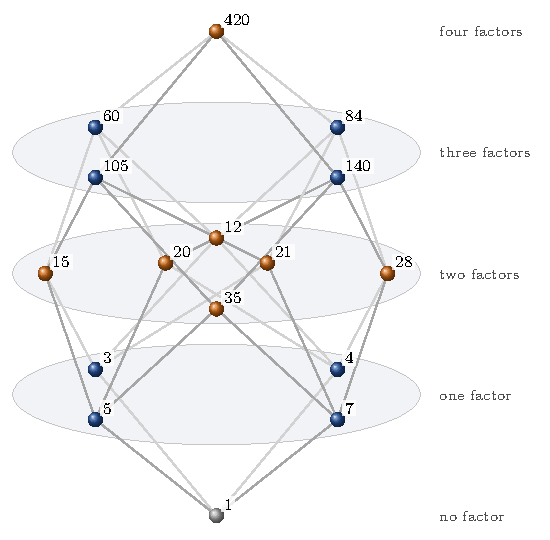
\includegraphics[width=0.72\textwidth]{figures/fig_aoki}
\caption{The products of distinct elements of $\mathsf P$ that divide
$2^{a}3^{b}5^{c}7^{d}$ for large exponents, arranged by the number of
factors, with an edge for each added factor. The products of an even number
of factors, in orange, form $\mathcal Q(M)$; each carries one class
$\xi_{q}$ of \Cref{thm:aoki}.}\label{fig:aoki}
\end{figure}

\begin{theorem}[Aoki]\label{thm:aoki}
For every $q\in\mathcal Q(M)$ there is an element $\xi_{q}\in B_{q}$ such that
\[
  B_{M}=S_{M}+\sum_{q\in\mathcal Q(M)}\ \sum_{t\in(\ZZ/M)^{\times}}
  \ZZ\,t\cdot(M/q)_{*}\xi_{q}.
\]
Moreover $2x\in S_{M}$ and $x+t\cdot x\in S_{M}$ for every $x\in B_{M}$ and
every unit $t$.
\end{theorem}

This is \cite[Theorem~2.1]{Aok00}; the second assertion is part of the proof
of \cite[Corollary~2.3]{Aok00}. It rests on \cite[Theorem~D]{Aok83}, where
the groups are normalized differently; Peterson explains the translation
\cite[\S5.2]{Pet26}.\footnote{Aoki also shows that $B_{M}/S_{M}\cong
(\ZZ/2)^{|\mathcal Q(M)|}$ \cite[Remark~2.4]{Aok00}, so that none of the
classes $\xi_{q}$ can be omitted. For $M=p^{e}$ and $M=2p^{e}$, with $p$ an
odd prime, $\mathcal Q(M)$ is empty, and \Cref{thm:aoki} with
\Cref{lem:transfer} gives the Hodge conjecture for $X^{n}_{M}$ in every
dimension, a theorem of Aoki \cite{Aok87,Aok00}.} We use it through the
following two consequences. Say that a level $M$ is \emph{complete} if every
balanced multiset of an even number of nonzero elements of $\ZZ/M$ is
algebraic. A complete level has the Hodge conjecture for $X^{n}_{M}$ in every
dimension $n$, by the end of the proof of \Cref{lem:transfer}, and every
divisor of a complete level is complete, by \Cref{lem:algtools}(d).

\begin{proposition}\label{prop:complete}
Let $M\ge3$. If every $q\in\mathcal Q(M)$ is a complete level, then $M$ is
a complete level.
\end{proposition}

\begin{proof}
Each $\xi_{q}\in B_{q}$ is an integral combination of classes of balanced
multisets with an even number of elements, which are algebraic as $q$ is
complete. By \Cref{lem:algtools}(c),(d), $t\cdot(M/q)_{*}\xi_{q}$ is then an
integral combination of classes of algebraic balanced multisets at level
$M$. \Cref{thm:aoki} and \Cref{lem:transfer} give the claim.
\end{proof}

\begin{corollary}\label{cor:Bone}
Suppose that $\mathcal Q(M)$ has exactly one element, and let $\nu\colon
R_{M}\to\ZZ/2$ be a homomorphism that vanishes on $S_{M}$. If $\beta$ is a
balanced multiset of an even number of nonzero elements of $\ZZ/M$ with
$\nu([\beta])=1$, then $B_{M}=S_{M}+\ZZ[\beta]$. This applies to
\[
\begin{array}{@{}l@{\qquad}l@{}}
  M=114,\ \nu=\nu_{19},\ \mathcal Q=\{57\}; & M=102,\ \nu=\nu_{17},\
  \mathcal Q=\{51\};\\
  M=44,\ \nu=\nu_{11},\ \mathcal Q=\{44\}; & M=52,\ \nu=\nu_{13},\
  \mathcal Q=\{52\};\\
  M\in\{33,35,39\},\ \nu=\nu_{R},\ \mathcal Q=\{M\}. &
\end{array}
\]
\end{corollary}

\begin{proof}
Let $\mathcal Q(M)=\{q\}$. By \Cref{thm:aoki}, $B_{M}/S_{M}$ is generated by
the images of the elements $t\cdot(M/q)_{*}\xi_{q}$, and $t\cdot x\equiv-x
\equiv x$ modulo $S_{M}$ for every $x\in B_{M}$. So $B_{M}/S_{M}$ is
generated by one element of order at most $2$. As $\nu([\beta])=1$,
$[\beta]\notin S_{M}$; hence $B_{M}/S_{M}$ has order $2$ and is generated by
the image of $[\beta]$. The homomorphisms named vanish on $S_{M}$ by
\Cref{lem:nu,lem:nusqrt}. The elements of $\mathsf P$ that divide
$114=2\cdot3\cdot19$ are $3$ and $19$, those dividing $102=2\cdot3\cdot17$
are $3$ and $17$, since $2\notin\mathsf P$, those dividing $44=4\cdot11$ and
$52=4\cdot13$ are $4,11$ and $4,13$, and those dividing $33$, $35$, $39$ are
their two prime factors; this gives the values of $\mathcal Q$.
\end{proof}

\subsection{Aoki's degrees}
Aoki proves the Hodge conjecture for every abelian variety of Fermat type of
degree $m$ when $m=2^{a}3^{b}5^{c}7^{d}$ with $c=0$ or $d=0$, and when $m$ is
$p^{e}$ or $2p^{e}$ for a prime $p$ \cite[Theorem~0.1]{Aok00}. Among these
abelian varieties are the powers of the Jacobian of the Fermat curve
$X^{1}_{m}$, and the Fermat varieties of degree $m$ are built from that
curve.

\begin{lemma}\label{lem:abelianfermat}
Let $m\ge1$, let $J$ be the Jacobian of $C=X^{1}_{m}$, and suppose that the
Hodge conjecture holds for $J^{N}$ for every $N$. Then it holds for
$X^{n}_{m}$ for every $n$.
\end{lemma}

\begin{proof}
First, the Hodge conjecture holds for $C^{N}$. Fix $o\in C$ and let
$\iota\colon C\to J$ be the Abel--Jacobi map $x\mapsto[x-o]$; then
$\iota^{*}\colon H^{1}(J)\to H^{1}(C)$ is an isomorphism of Hodge
structures. By the K\"unneth formula, $H^{*}(C^{N})$ is the direct sum of
the sub-Hodge structures $H_{T,V}$, indexed by disjoint subsets $T,V$ of
$\{1,\dots,N\}$, that are the tensor products of $H^{1}(C)$ at the factors in
$T$, of $H^{2}(C)=\QQ[o]$ at those in $V$ and of $H^{0}(C)$ at the others. A
Hodge class $h$ of $C^{N}$ is the sum of its components $h_{T,V}$, which are
Hodge classes, and $h_{T,V}=\pr_{T}^{*}g\cup\prod_{i\in V}\pr_{i}^{*}[o]$
for a Hodge class $g$ in the summand $H^{1}(C)^{\otimes T}$ of
$H^{|T|}(C^{T})$. This summand is the image, under the isomorphism
$(\iota^{T})^{*}$, of the summand $H^{1}(J)^{\otimes T}$ of $H^{|T|}(J^{T})$,
so $g=(\iota^{T})^{*}g'$ for a Hodge class $g'$ on $J^{T}$, which is
algebraic. So $g$ and $h_{T,V}$ are algebraic.

Next, write $X^{j}=X^{j}_{m}$. We show by induction on $j$ that the Hodge
conjecture holds for $C^{k}\times X^{j}$ for every $k$; $X^{0}$ is a set of
$m$ points and $X^{1}=C$, so the cases $j\le1$ are the first step. Let
$j\ge2$, and let $\psi\colon Z\to X^{j}$ be the morphism of the inductive
structure with $r=1$ and $s=j-1$, so that $Z$ is the blow-up of $C\times
X^{j-1}$ along $Y\cong X^{0}\times X^{j-2}$. Then $W=C^{k}\times Z$ is the
blow-up of $C^{k+1}\times X^{j-1}$ along $C^{k}\times Y$, a disjoint union
of $m$ copies of $C^{k}\times X^{j-2}$, of codimension two. By the blow-up
formula \cite[Theorem~7.31]{Voi02b}, the map
\[
  H^{i}(C^{k+1}\times X^{j-1})\oplus H^{i-2}(C^{k}\times Y)(-1)\to
  H^{i}(W),
\]
given by the pull-back and by the pull-back to the exceptional divisor
followed by the push-forward, is an isomorphism of Hodge structures. Both
components carry algebraic classes to algebraic classes, so by
\Cref{lem:lift} and induction the Hodge conjecture holds for $W$. The
morphism $\phi=\mathrm{id}\times\psi\colon W\to C^{k}\times X^{j}$ is
surjective between varieties of the same dimension, and
$\phi_{*}\phi^{*}$ is multiplication by its degree. So a Hodge class $h$ of
$C^{k}\times X^{j}$ is $(\deg\phi)^{-1}\phi_{*}\phi^{*}h$, and $\phi^{*}h$
is algebraic. The case $k=0$ is the claim.
\end{proof}

\begin{proposition}\label{prop:aokidegrees}
Every level $m=2^{a}3^{b}5^{c}7^{d}$ with $c=0$ or $d=0$ is complete. In
particular $12$, $15$, $20$, $21$ and $28$ are complete levels.
\end{proposition}

\begin{proof}
The powers of $J$ are abelian varieties of Fermat type of degree $m$, so
\cite[Theorem~0.1]{Aok00} and \Cref{lem:abelianfermat} give the Hodge
conjecture for $X^{n}_{m}$ for every $n$. If $A$ is a balanced multiset of
$n+2$ nonzero elements of $\ZZ/m$, the line $V(\alpha)$ of
\Cref{prop:fermatchars}(ii) consists of Hodge classes of $X^{n}_{m}$, hence
of algebraic classes.
\end{proof}
